\qquad A análise de complexidade do Insertion Sort, considerando as
diferentes situações de entrada (crescente, decrescente e
randômica), foi realizada manuscrita, com a devida justificativa,
conforme exigido pelo enunciado do trabalho. A digitalização do
material manuscrito deve ser inserida a seguir, substituindo a
imagem de exemplo abaixo.

\begin{figure}[htbp]
    \centering
    % Substitua o arquivo abaixo pela digitalizacao da analise de complexidade manuscrita
    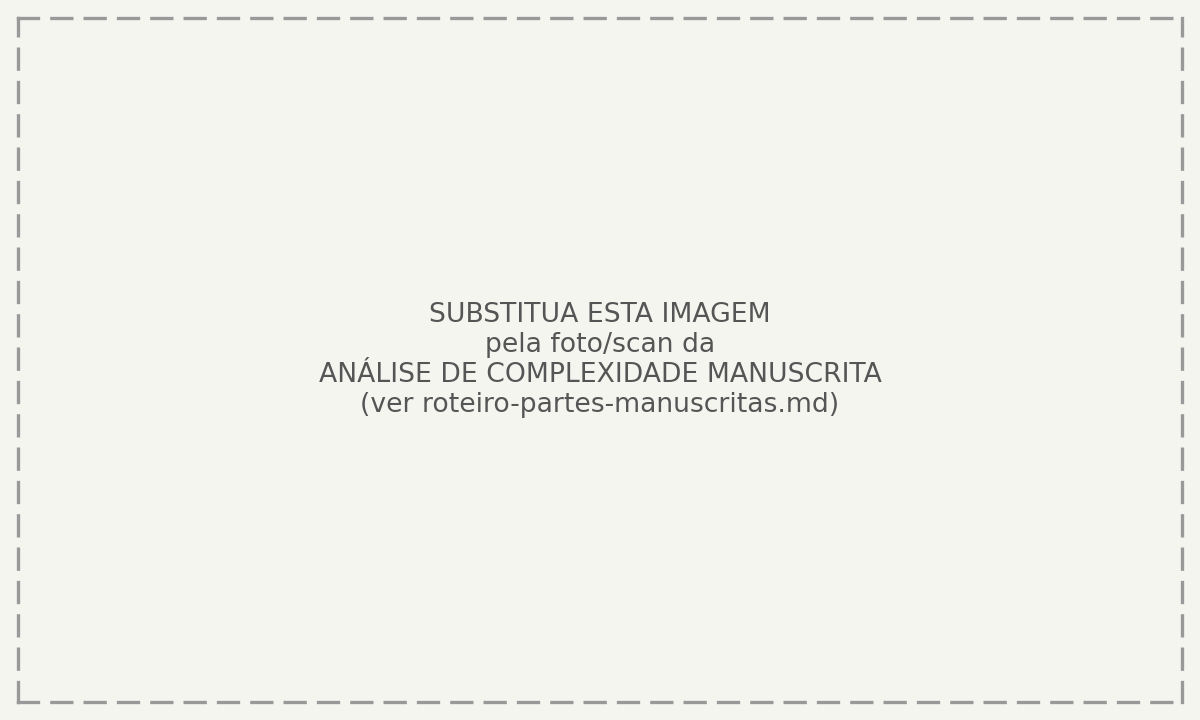
\includegraphics[width=14cm]{Imagens/Insertion Sort/analise_complexidade.png}
    \caption{Análise de complexidade manuscrita do algoritmo Insertion Sort}
    \label{fig:analise_complexidade}
\end{figure}

\qquad Os resultados experimentais apresentados na próxima seção deste
capítulo são compatíveis com essa análise teórica: desempenho linear
no melhor caso (entrada crescente) e desempenho quadrático no caso
médio e no pior caso (entradas randômica e decrescente).
